% !TEX TS-program = pdflatexmk
\documentclass{./packages/optica-article}

\graphicspath{{images/}{practica2/images}}

\journal{opticajournal}
\usepackage{csvsimple}
\usepackage{siunitx}
\usepackage{physics}
\usepackage{booktabs}
\usepackage{tikz}

\usepackage{caption}
\usepackage{subcaption}

% No floating captions
\usepackage{capt-of}
\usetikzlibrary{positioning}

\tikzset{>=stealth}

% cref instead of ref
\usepackage{cleveref}

\newcommand{\sinc}{\textrm{sinc}}
\newcommand\conv{\circledast}

% Set the article type
\articletype{Research Article}

% \usepackage{lineno}
% \linenumbers

\begin{document}

\title{El efecto Talbot}

\author{Adriana Mamani Lazarte\authormark{1} Alex G. Recuenco\authormark{1}, and Carlos España Castaño\authormark{1}}

\address{\authormark{1}Universidad Complutense de Madrid, Madrid, PC 28040, España}

\section{Introducción}
En la práctica realizada primeramente se aprendió a realizar montajes experimentales de sistemas ópticos, de tal manera que el mismo este alineado de manera correcta y el haz se encuentre colimado. Se estudia experimentalmente el efecto de Talbot que es la reproducción de campos periódicos durante la propagación en el espacio
libre en el régimen de Fresnel para ciertas distancias. Por otra parte, se construyó un sistema para la observación y medida del espectro de Fourier de un objeto 2D (en este caso una lámina fotográfica). Se analiza la difracción de la iluminación coherente de una imagen al mover la cámara con respecto a la imagen.

\section{Desarrollo}

\subsection{Marco Práctico}
    \begin{enumerate}
    \item Observación efecto de Talbot\\
La primera parte de la práctica consistió en la observación de imágenes de la difracción de una onda plana coherente y monocromática en el régimen de Fresnel por un objeto periódico. 
Se trabajó con un láser de 635nm , en el siguiente sistema en la cual la lente colimadora transforma la onda esférica divergente en una onda plana.:

% Nota como para FORZARLO a estar aqui, no se utiliza figure, que es algo que flota
% Esto normalmente esse considera mala forma en un documento, ya que LaTeX es muy bueno a cuadrar todo
\begin{center}
    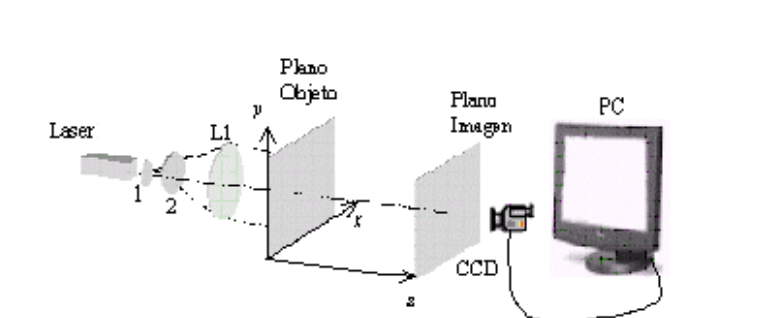
\includegraphics[scale=1]{sistematalbot.png}
     \captionof{figure}{Esquema del banco óptico, (1) filtro espacial, (2) atenuador, L1 lente colimadora, cámara CCD y PC para efectuar el registro.}
    \label{fig:talbot} % for use in \ref{table1} if you want to refer to the table number
\end{center}

    \item Espectro de Fourier

Para obtener el módulo de la transformada de Fourier de una escena mediante sistemas ópticos se trabajó con un montaje que se componía por una lente delgada, cuyo plano de entrada está iluminado por un plano de luz, coherente y monocromático. 

\begin{figure}[h]
    \centering
    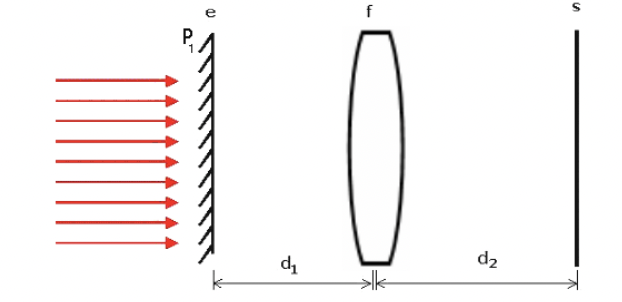
\includegraphics[scale=1]{sistemaespectrodefourier.png}
    \caption{Esquema del montaje experimental para la observación del espectro de Fourier de un objeto plano. }
    \label{fouriersistema}
    \end{figure}
    
En el sistema armado se utilizaron lentes focales diferentes, un polarizador como atenuador y un diafragma para disminuir la influencia de luz parasita.\\
Se observaron los espectros de Fourier en distintos escenarios que expondremos en la parte de resultados de la práctica.
    \item Filtrado óptico
Se realiza la práctica experimental de esta parte con el montaje de un sistema 4f introducido por Van der Lugt para el procesado óptico de información de 1963

\begin{figure}[h]
    \centering
    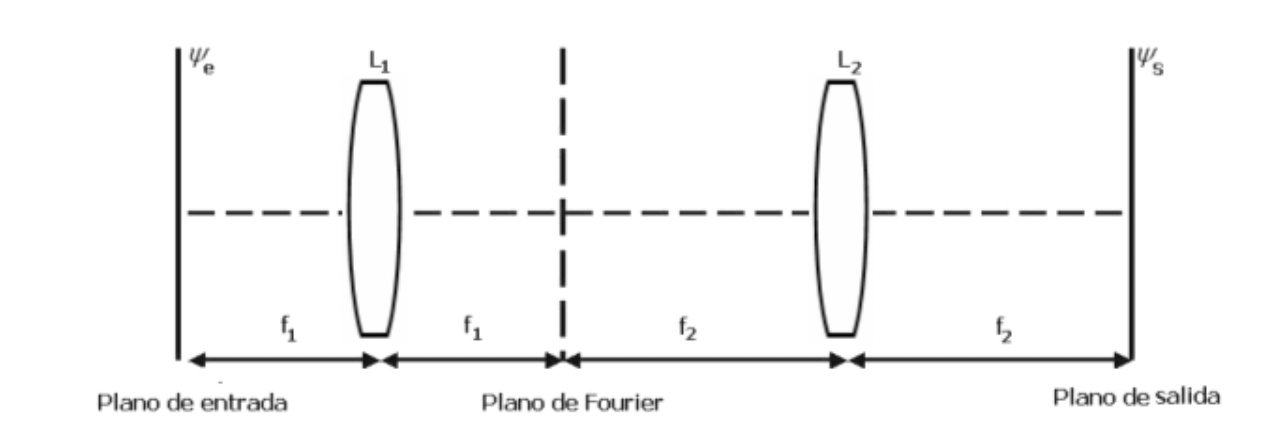
\includegraphics[scale=0.5]{/parte4-filtrado/Sistema3.png}
    \caption{Esquema para la realización de una operación de filtrado óptico.}
    \label{filtradoopticosistema}
    \end{figure}
    
Compuesto por un objeto de una escena en el plano P1, que es el focal de la lente L1 se ilumina con una onda plana. En el otro plano focal de la lente L1 donde se obtendrá la transformada de Fourier del objeto.

    \item Formación de imagen con luz parcialmente coherente

El grado de coherencia del haz afecta directamente a como un sistema óptico forma imagen, por lo tanto, controlaremos este parámetro. Por tanto, en el siguiente montaje con él trabajaremos.

\begin{figure}[h]
    \centering
    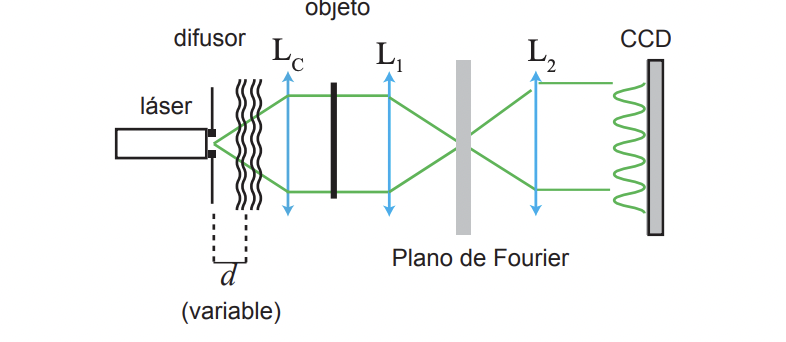
\includegraphics[scale=0.5]{/parte5-luz-coherente/sistema4.png}
    \caption{Esquema del montaje de la práctica}
    \label{coherenciaespacial}
    \end{figure}

\end{enumerate}

\section{Resultados experimentales}

\subsection{Observación del efecto Talbot}
Se observó la evolución del campo difractado al alejar la cámara CCD del plano del objeto, y se apuntó las distancias descritas a continuación:\\
Se registraron las imágenes y las distancias donde se observaron, 

\begin{figure}[hptb]
\begin{center}
    \begin{subfigure}[t]{0.45\textwidth}\centering
        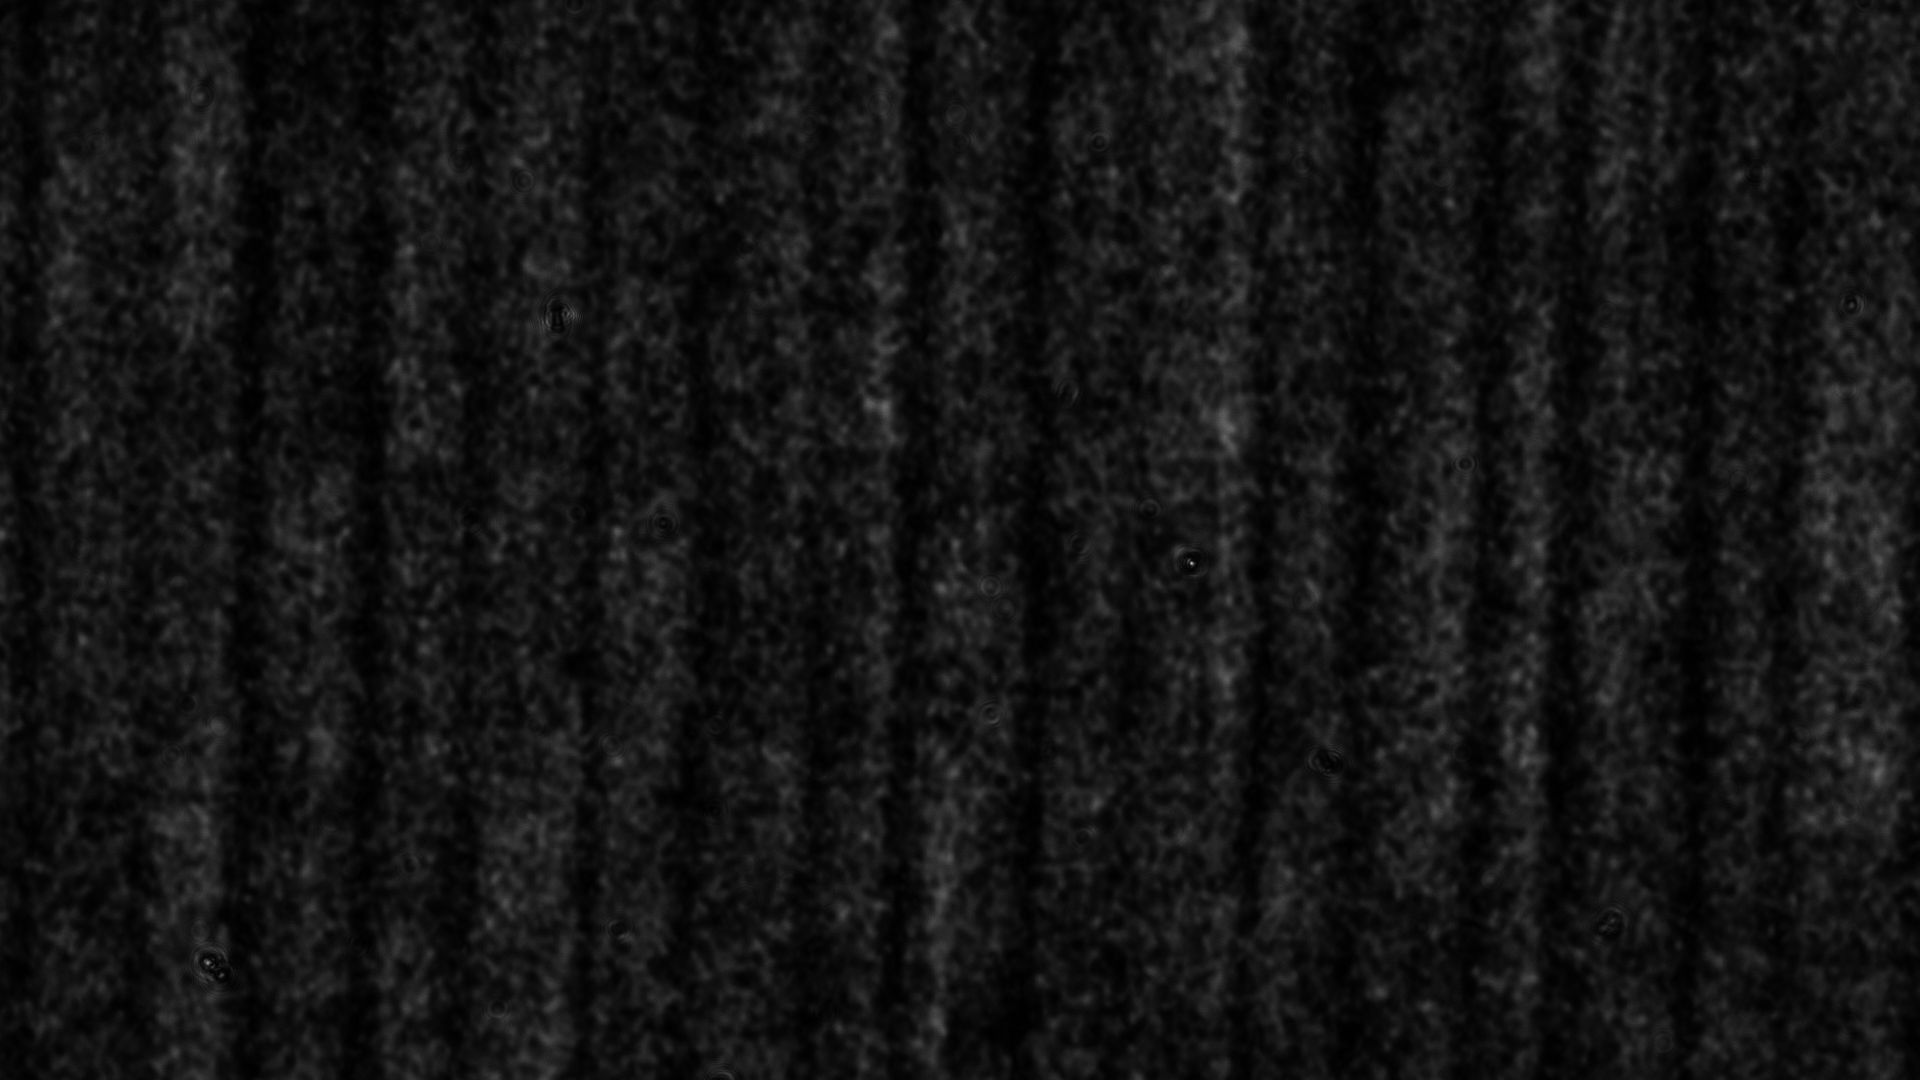
\includegraphics[width=\textwidth]{/parte2-talbot/4.9cm-talbot7.png}
        \caption{ Talbot a distancia 1}
        \label{fig:talbot1}	
    \end{subfigure}
	\hfill
	\begin{subfigure}[t]{0.45\textwidth}\centering
		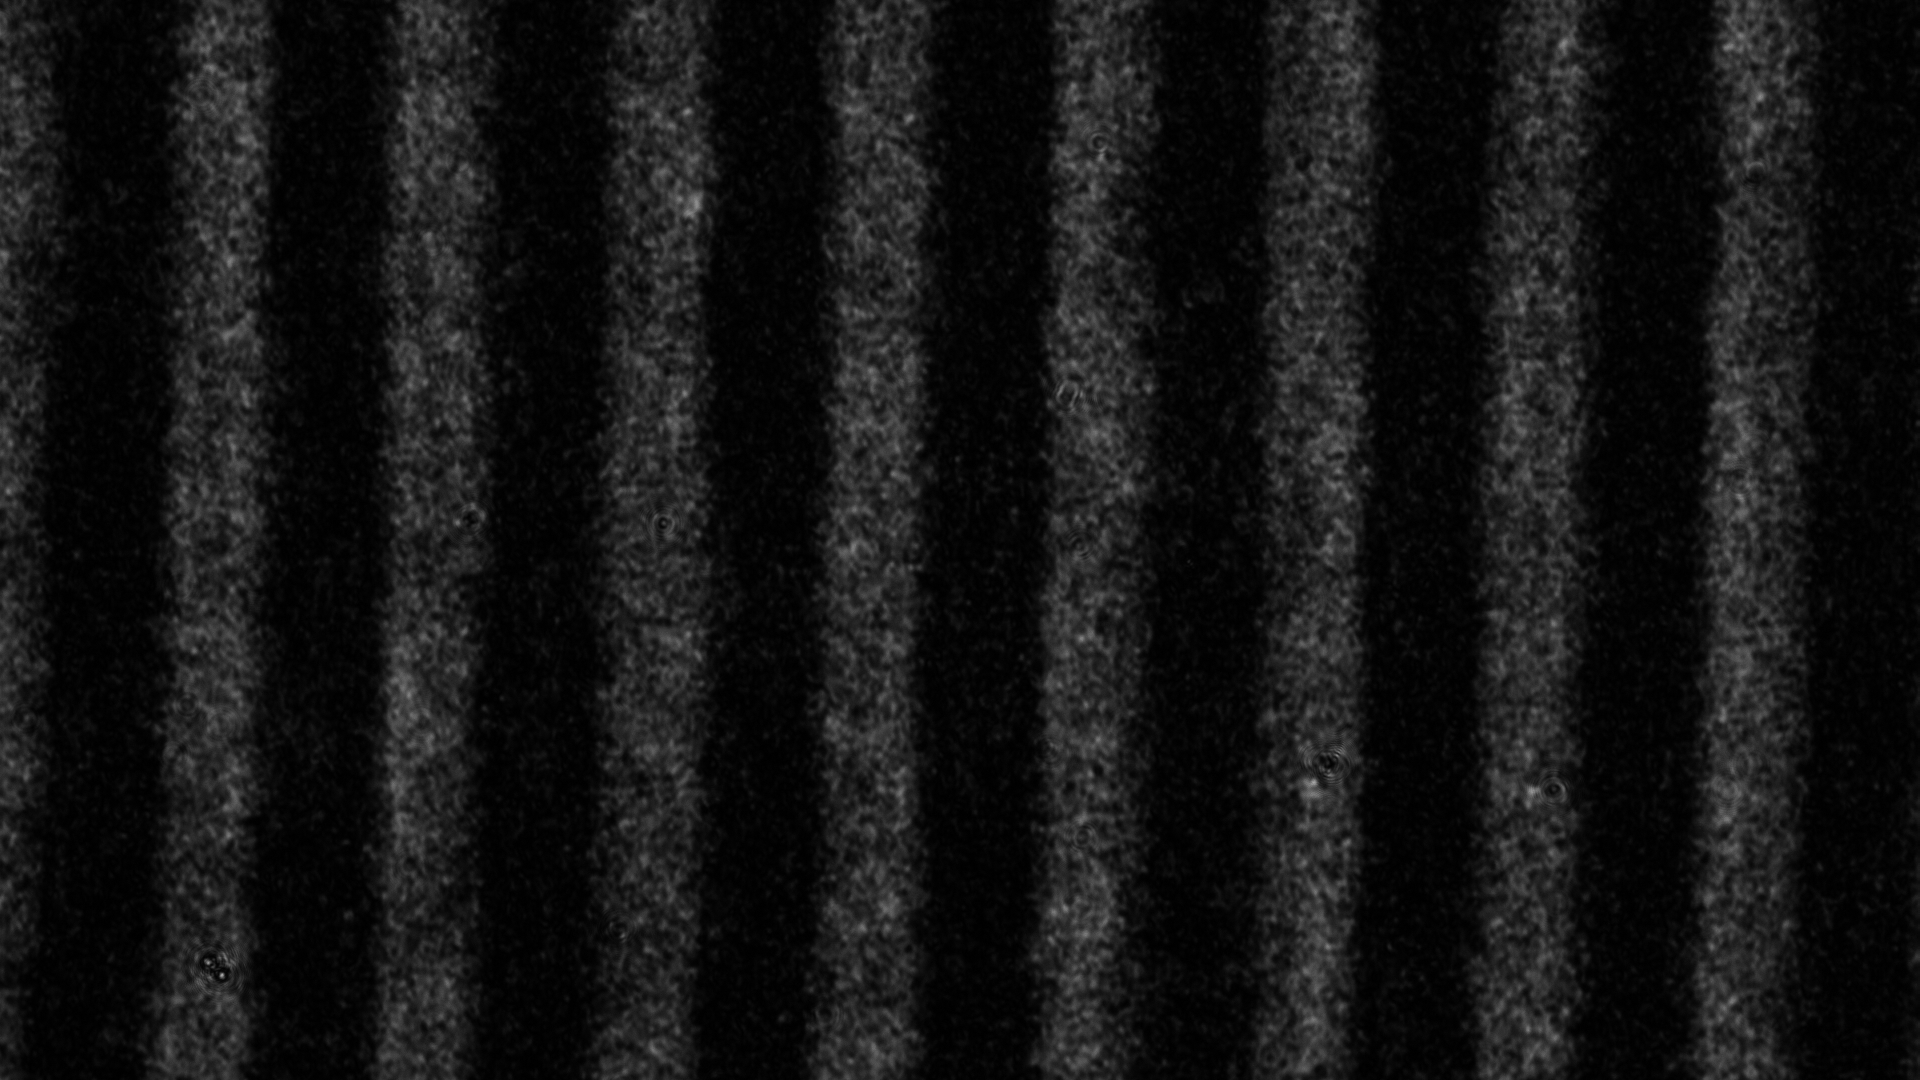
\includegraphics[width=\textwidth]{/parte2-talbot/23.9-talbot.png}
        \caption{Talbot a distancia 2}
        \label{fig:talbot2}
	\end{subfigure}
	\\
	\begin{subfigure}[t]{0.45\textwidth}\centering
		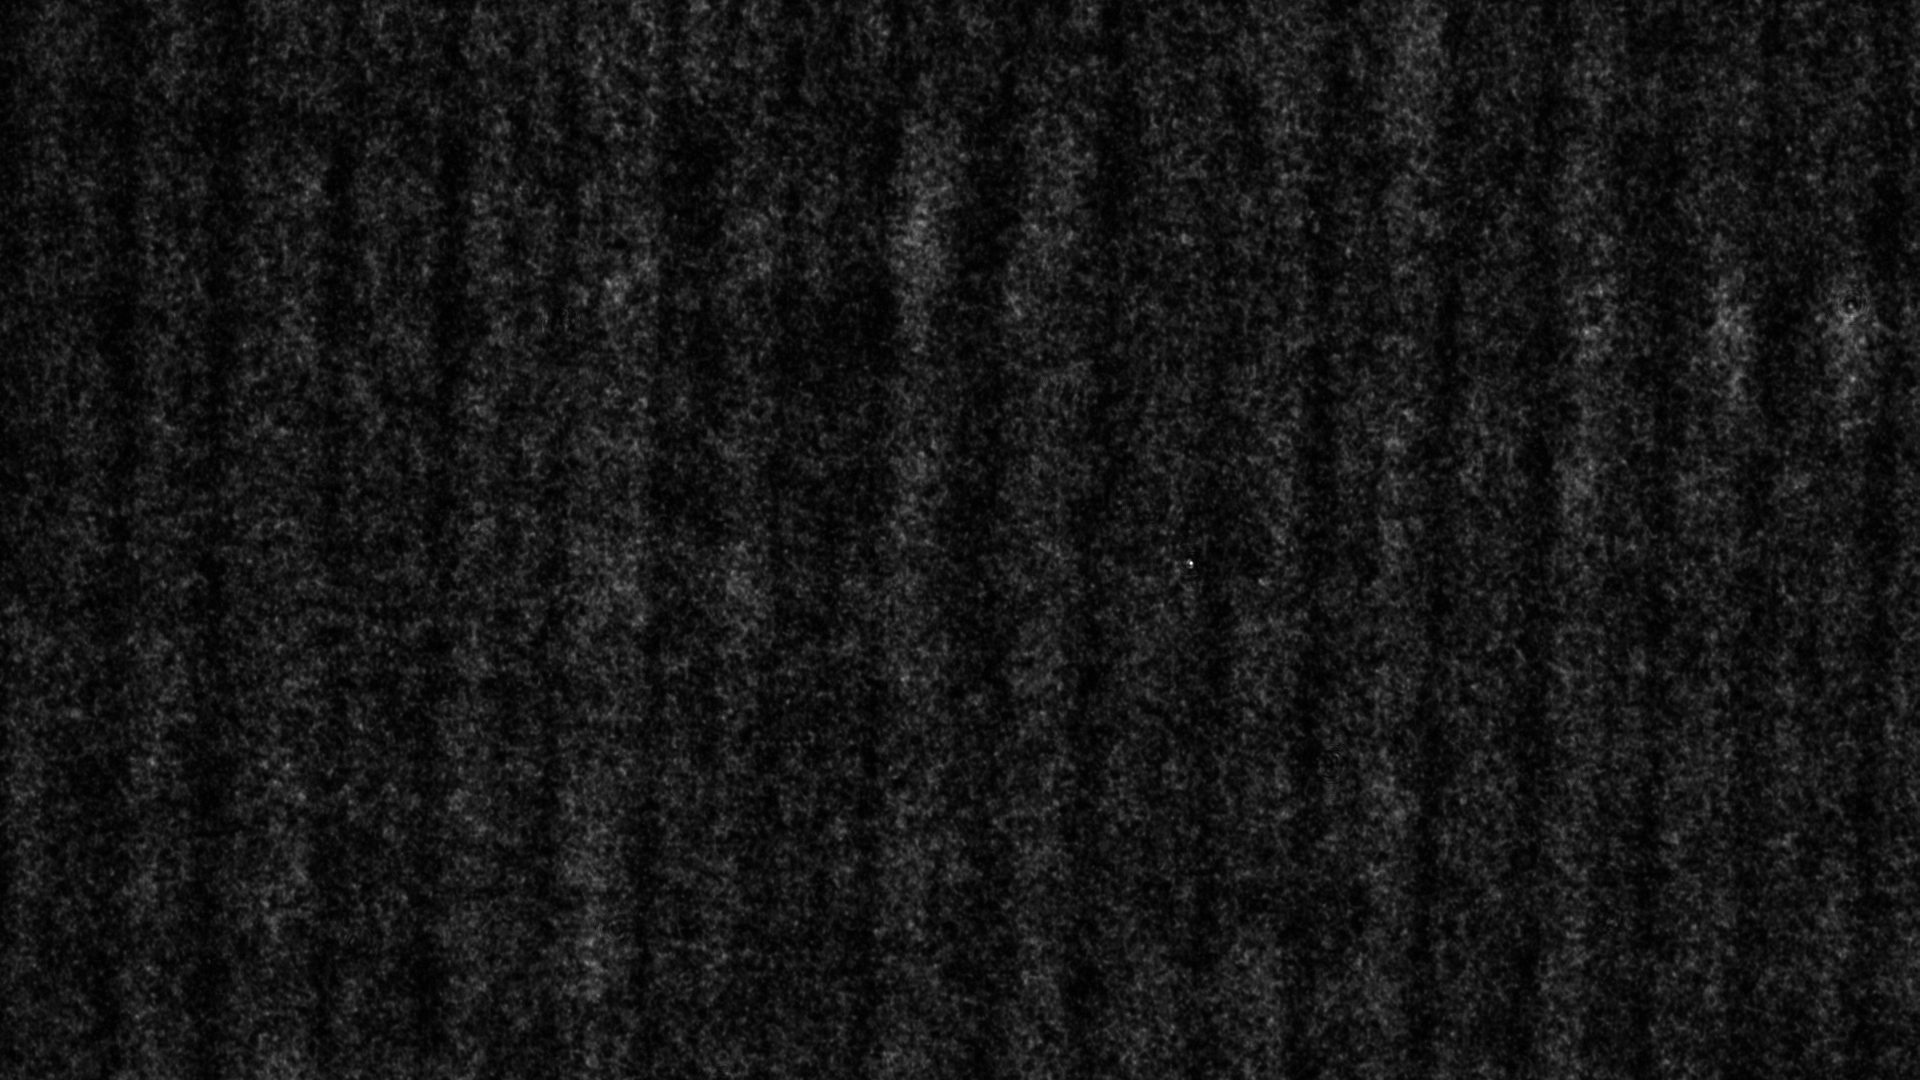
\includegraphics[width=\textwidth]{/parte2-talbot/42.2-talbot.png}
        \caption{ Talbot a distancia 3}
        \label{fig:talbot3}
	\end{subfigure}
	\hfill
	\begin{subfigure}[t]{0.45\textwidth}\centering
		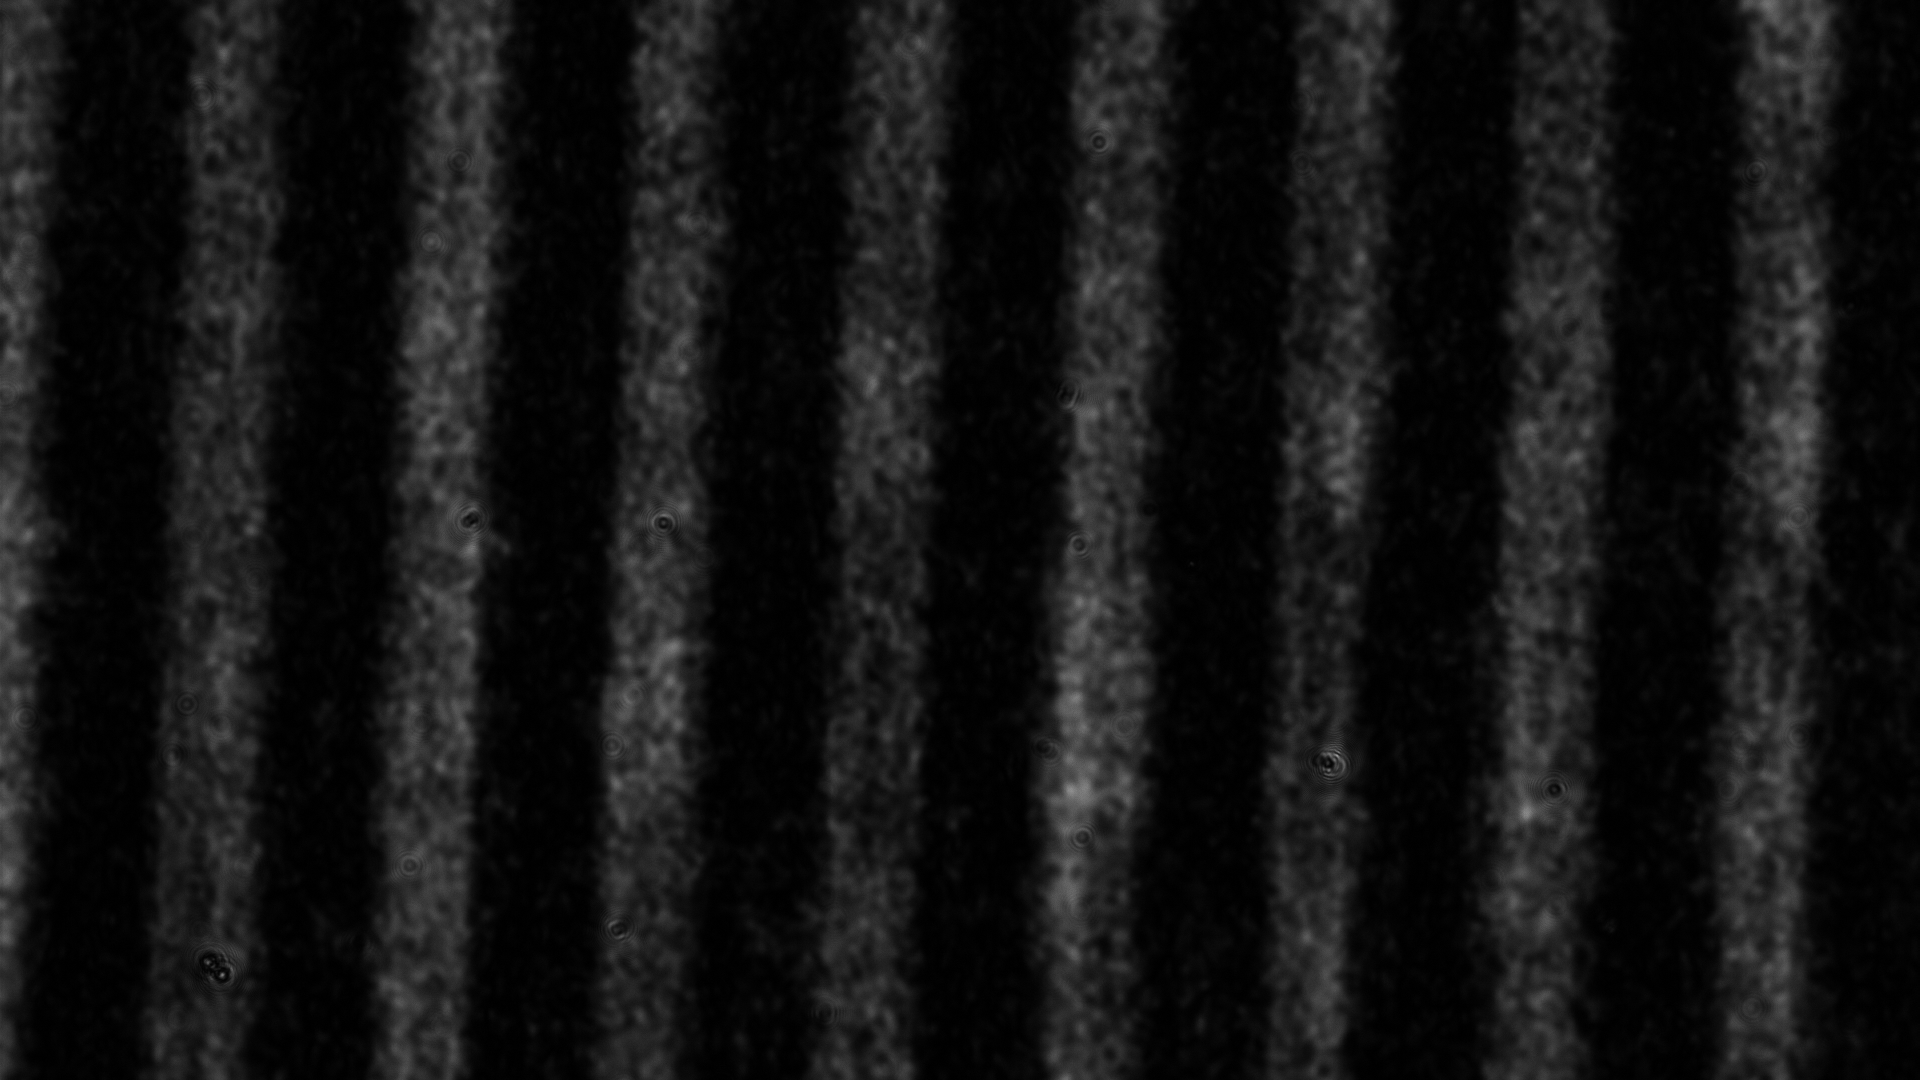
\includegraphics[width=\textwidth]{/parte2-talbot/54.8-2a-talbot.png}
        \caption{ Talbot a distancia 4}
        \label{fig:talbot4}
	\end{subfigure}
	
\caption{Posiciones de contraste máximo (\ref{fig:talbot2}, \ref{fig:talbot4}) y mínimo (\ref{fig:talbot1}, \ref{fig:talbot3})%
	}
	\label{fig:alltalbot}
\end{center}
\end{figure}

Distancia de Talbot: 

\begin{table}[h] % h indica que queremos posicionar la tabla Here
        \centering
        \begin{tabular}{|c|c|}
            \hline
            Distancia Imagen distribución de intensidad semejante & Distancia Imagen es semejante a la imagen original\\
            \hline
            18cm & 35,7cm\\
            \hline
            54cm & 73cm \\
            \hline
        \end{tabular}
        \caption{Distancias de Talbot}
        \label{tab:dtalbot}
    \end{table}
Periodo de la red:
d=\sqrt{\flatfrac{Z * \lambda}{2}}
Cuando una onda plana incide sobre una red de difracción periódica, la imagen de la red se repite a distancias regulares lejos del plano de la misma

\begin{table}[h] % h indica que queremos posicionar la tabla Here
        \centering
        \begin{tabular}{|c|c|}
            \hline
            Periodo Imagen distribución de intensidad semejante & Periodo Imagen es semejante a la imagen original\\
            \hline
            0.023cm & 0.34cm\\
            \hline
            0.41cm & 0,48cm \\
            \hline
        \end{tabular}
        \caption{Distancias de Talbot}
        \label{tab:dtalbot}
    \end{table}

CUESTIONES:
\begin{enumerate}
\item Representando una señal óptica periódica (longitud de onda $\lambda$, periodo $d$) como una serie de Fourier, demostrar analíticamente que en las distancias iguales a la mitad de la distancia de Talbot, $z=\flatfrac{ZT}{2}$, observamos el objeto original desplazado en la mitad del periodo $d$.

\item Usando las ecs. (7)-(8) analizar la intensidad y la fase del campo difractado por un objeto periódico compuesto de líneas blancas (transparentes) y negras (opacas) alternadas de la misma anchura, a una distancia $z=\flatfrac{ZT}{4}$

\item Justifique el procedimiento seguido para determinar la distancia de Talbot y el periodo de la red y exponga los resultados.

\item ¿Las imágenes observadas siempre son periódicos? \\¿La respuesta está de acuerdo con la teoría?
A distancias mayores a las de talbot mencionadas aparecen otras autoimágenes que no conservan su periodicidad axial.
\end{enumerate}

\subsection{Observación del espectro de Fourier}
Se toma los espectros de Fourier de las imágenes en cuestión presentadas a continuación:

\begin{figure}[hptb]
\begin{center}
    \begin{subfigure}[t]{0.45\textwidth}\centering
        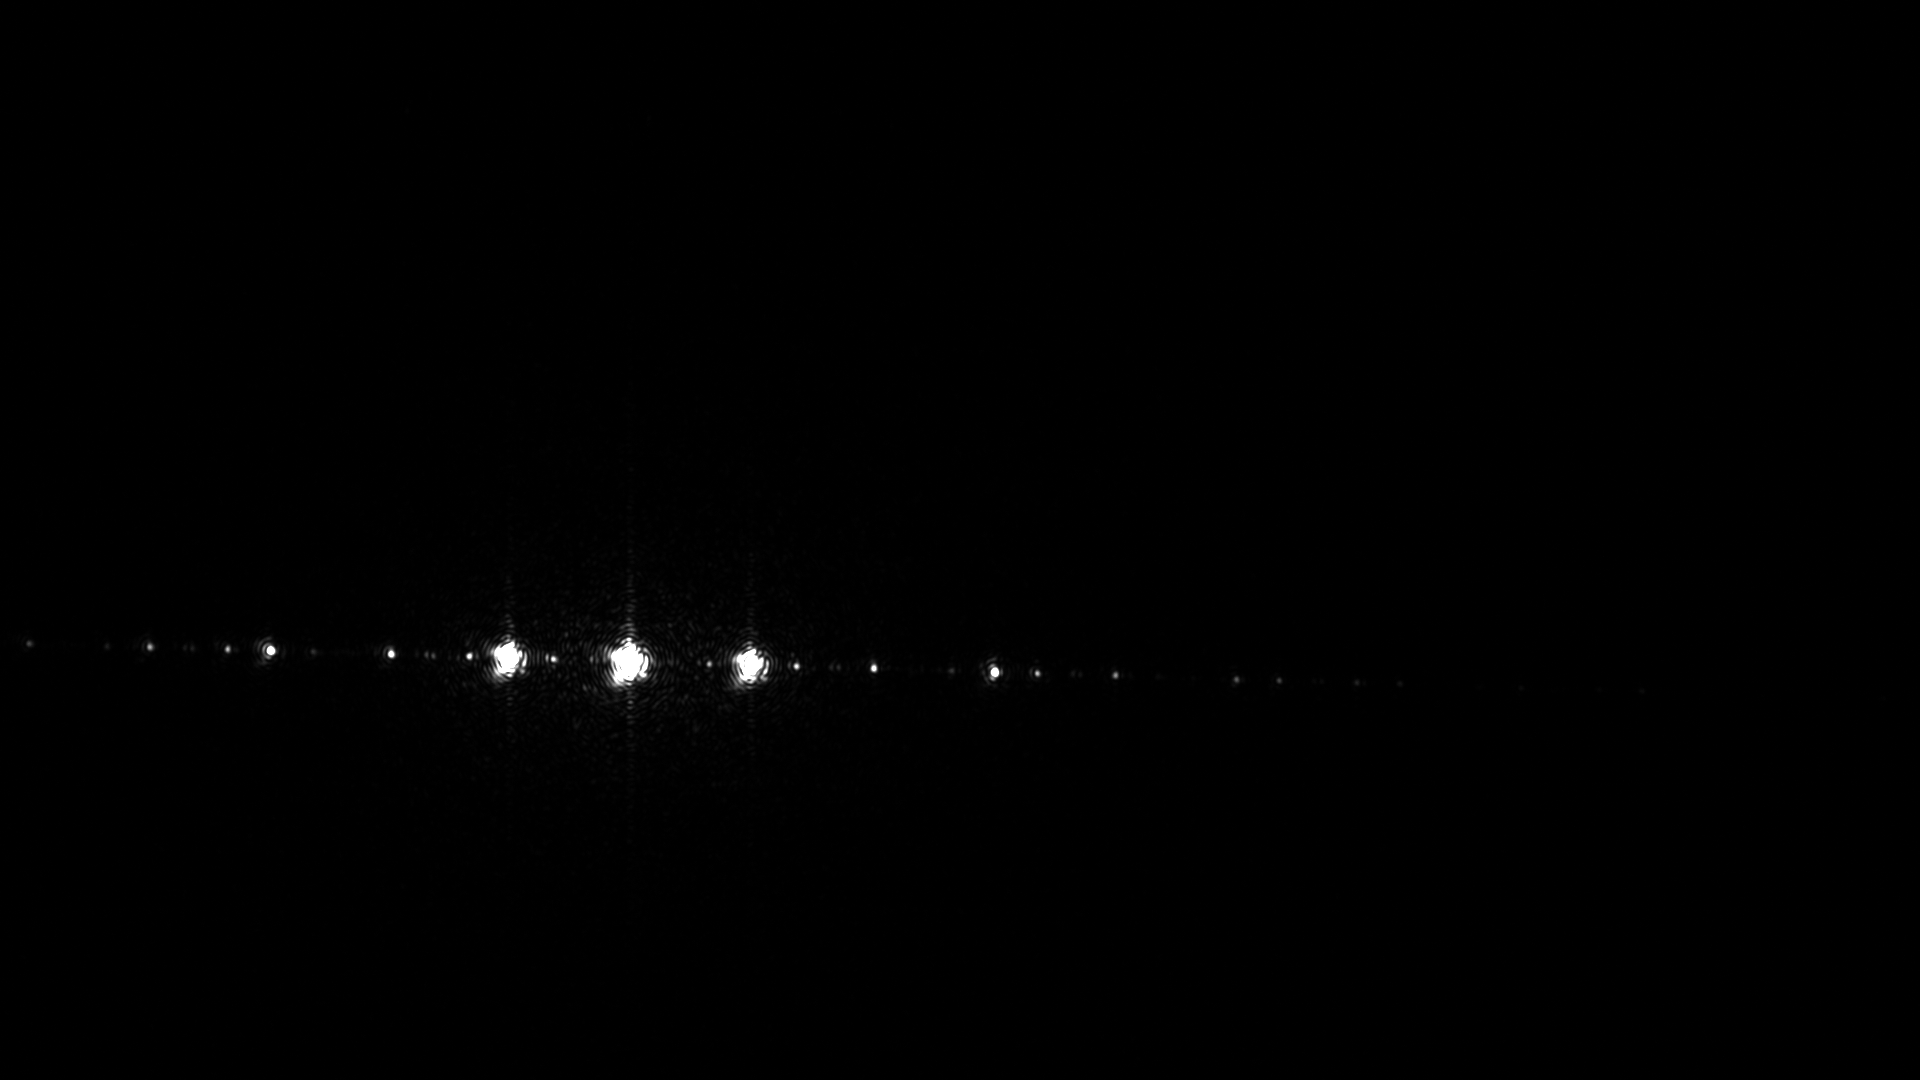
\includegraphics[width=\textwidth]{/parte3-fourier/fourier_transform_-20-lense-20-camera.png}
    \caption{Esquema del montaje experimental para la observación del espectro de Fourier de un objeto plano. }
    \label{fig:fourier1}
    \end{subfigure}
	\hfill
	\begin{subfigure}[t]{0.45\textwidth}\centering
		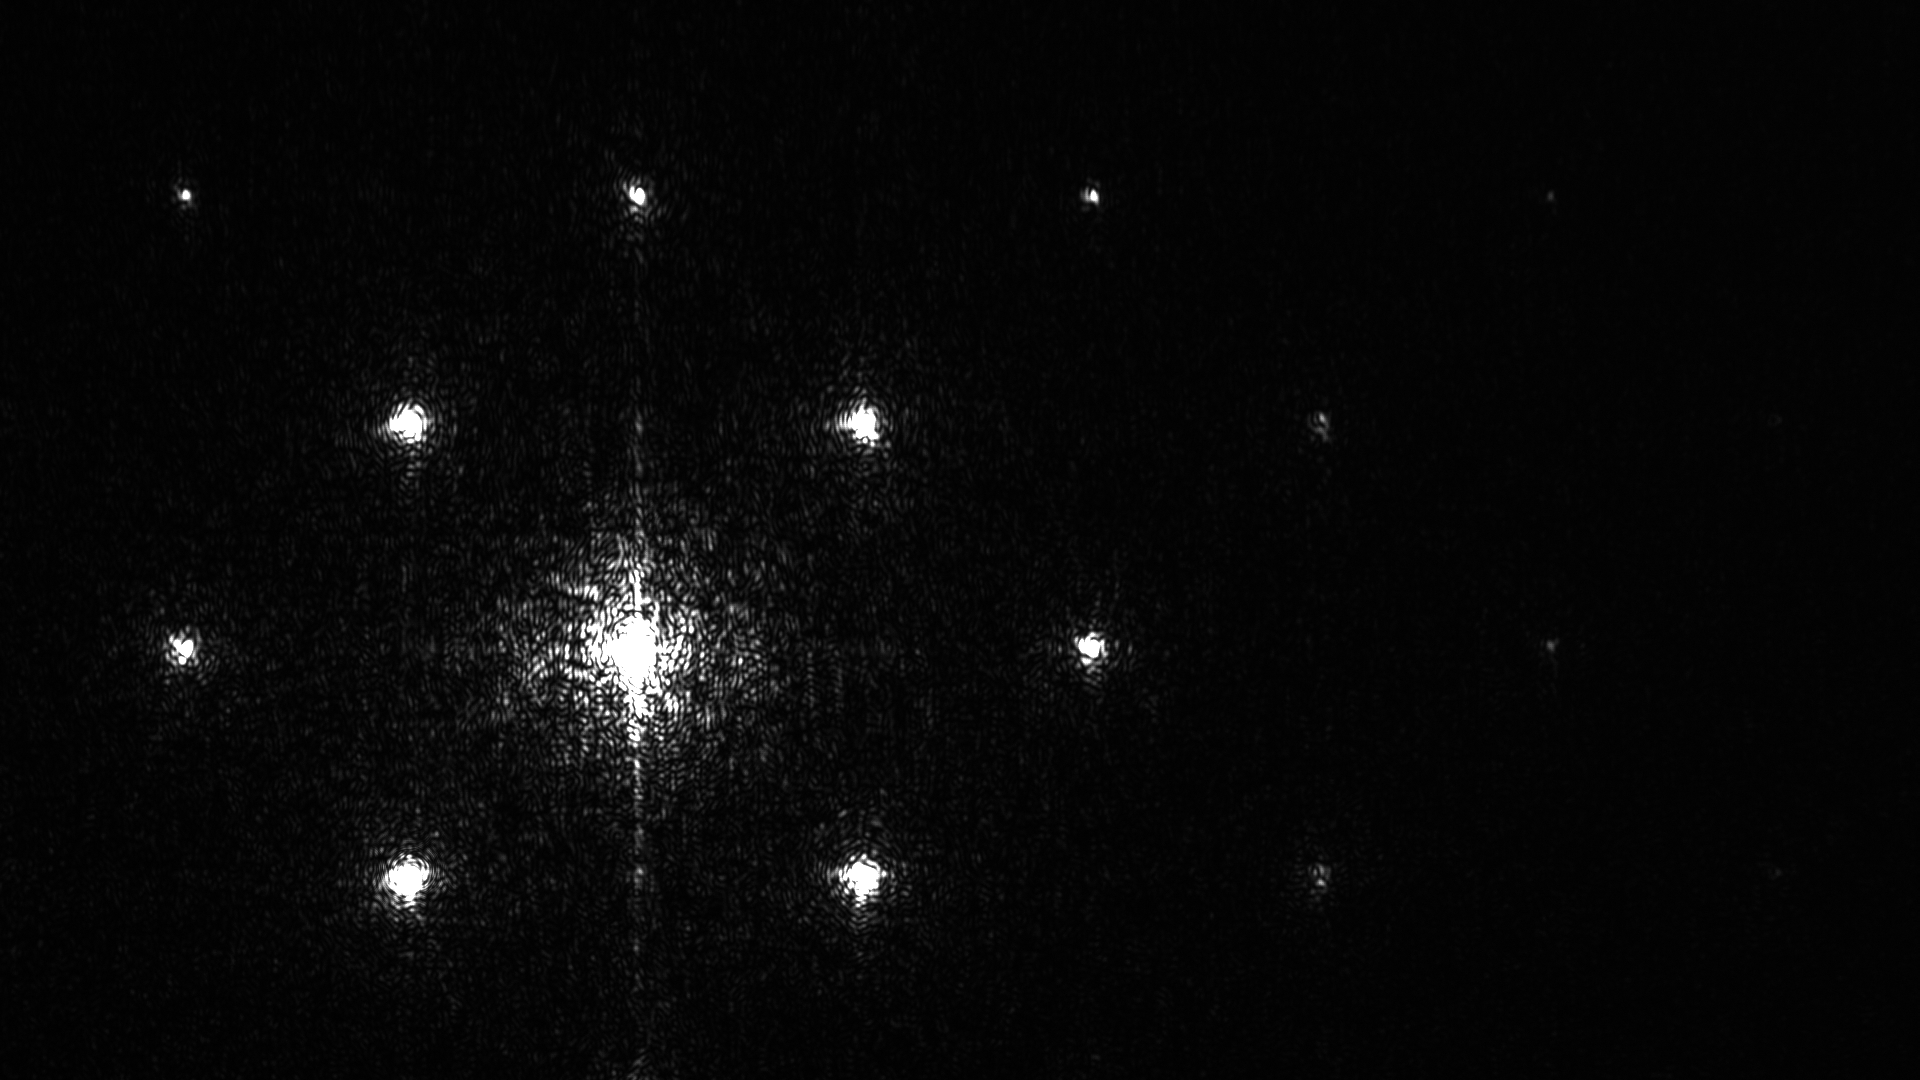
\includegraphics[width=\textwidth]{/parte3-fourier/fourier-car-multiplied-pixels.png}
    \caption{Espectro de Fourier imagen autos }
    \label{fig:fourier2}
	\end{subfigure}
	\\
	\begin{subfigure}[t]{0.45\textwidth}\centering
		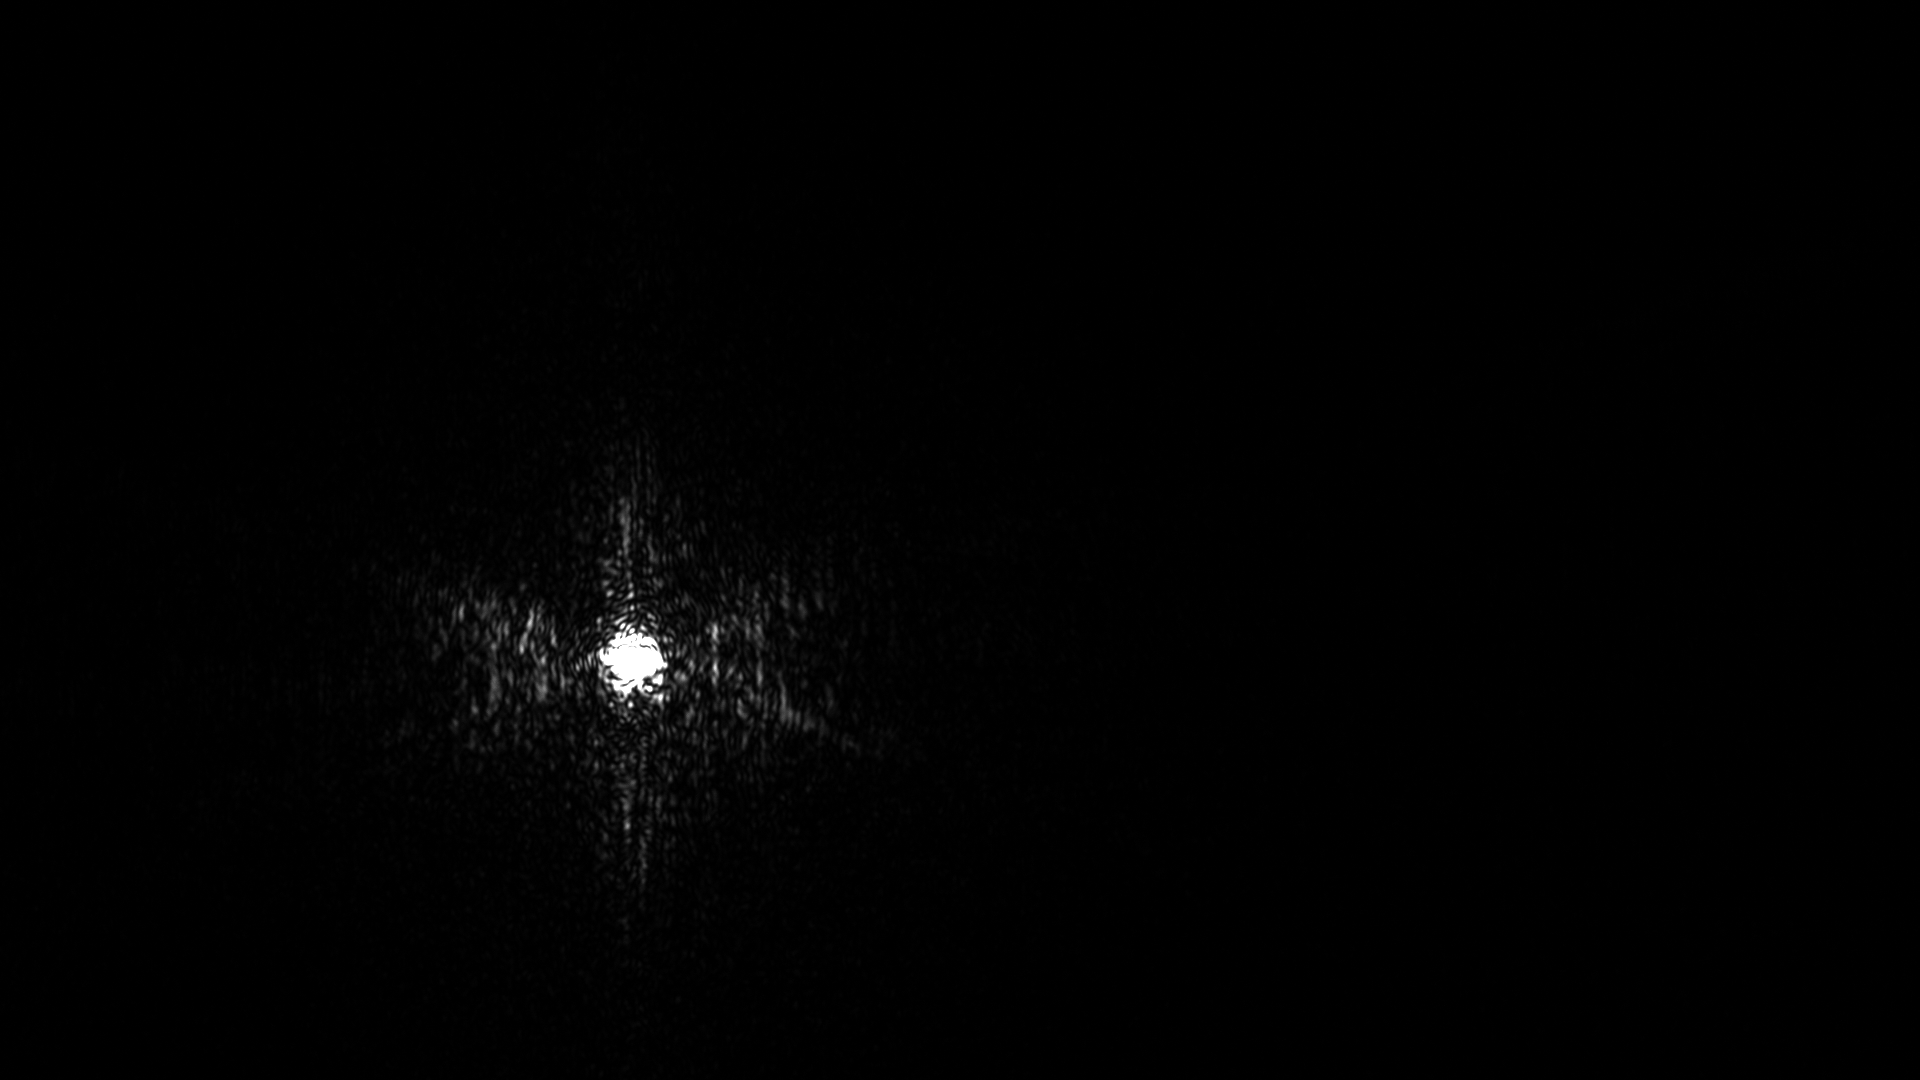
\includegraphics[width=\textwidth]{/parte3-fourier/fourier-letras.png}
    \caption{Espectro de Fourier imagen letras. }
    \label{fourier3}
	\end{subfigure}
	\hfill
	\begin{subfigure}[t]{0.45\textwidth}\centering
		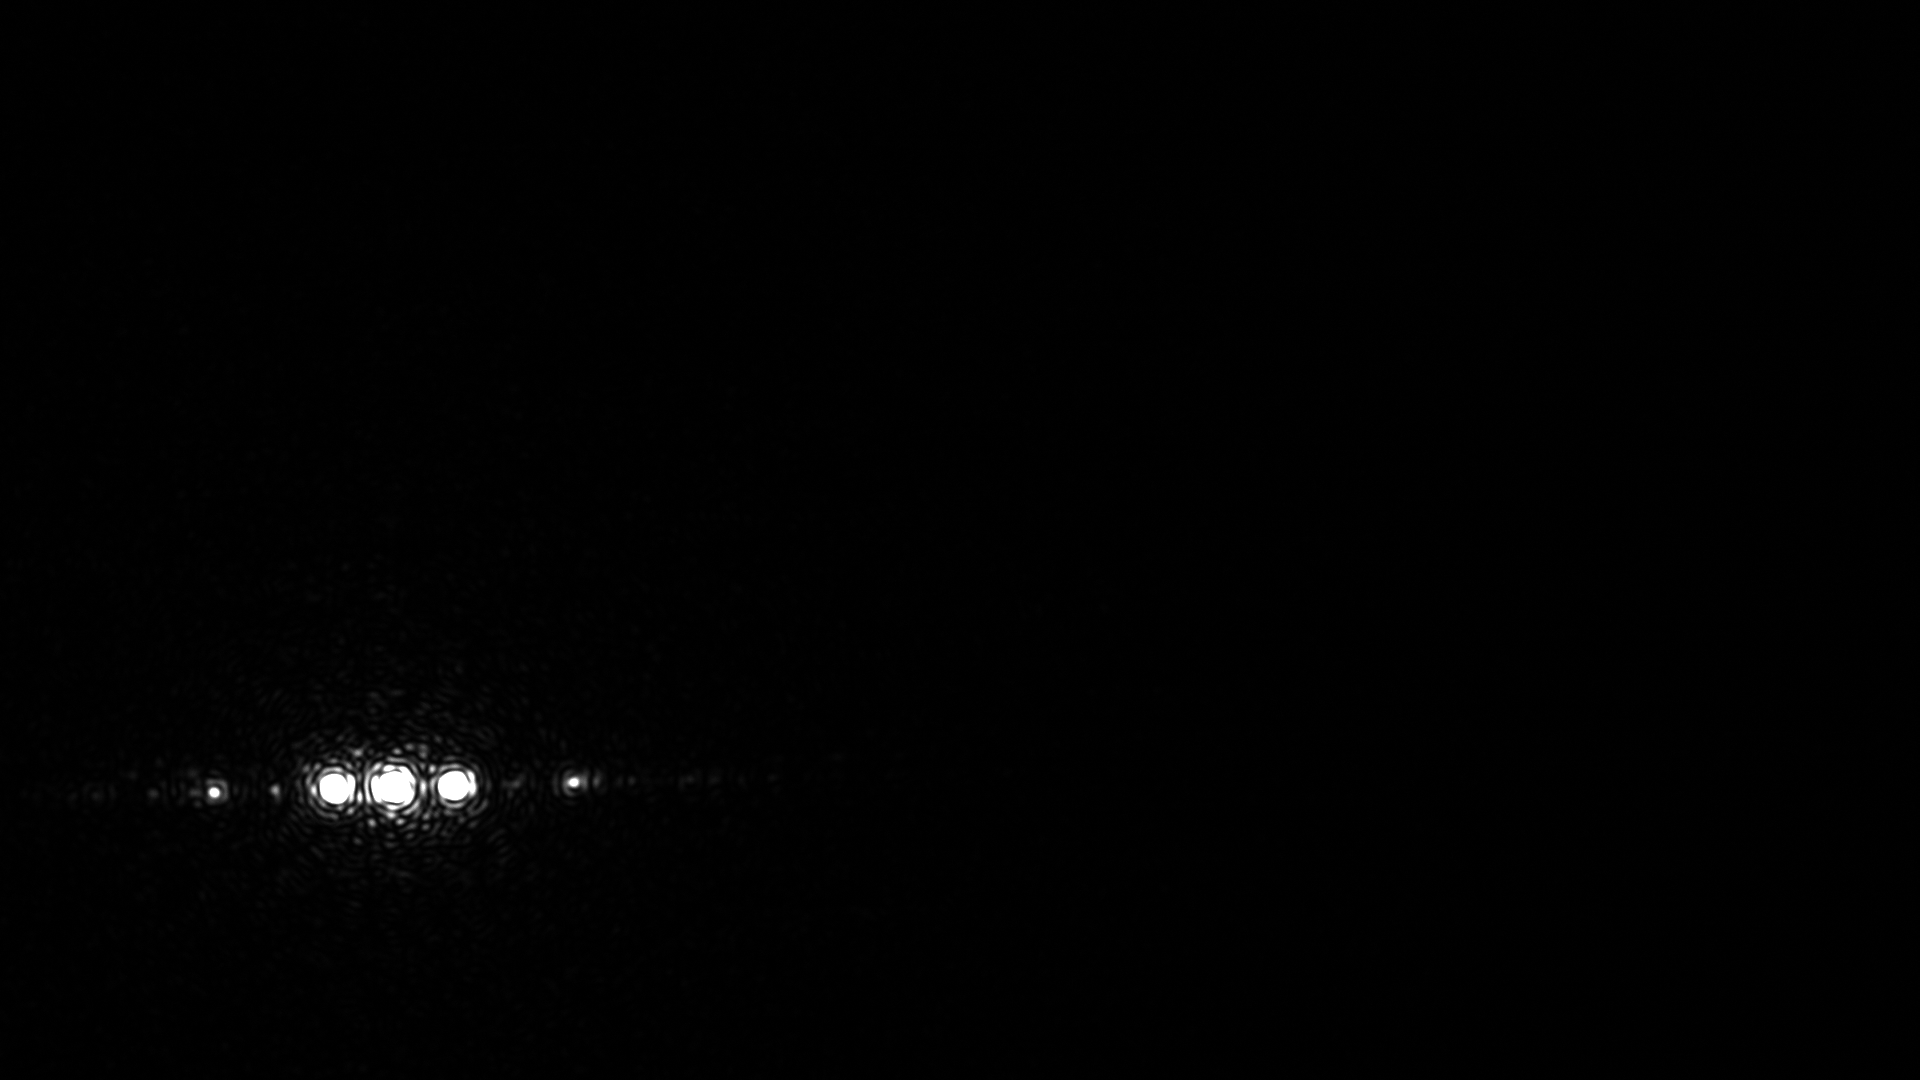
\includegraphics[width=\textwidth]{/parte3-fourier/fourier-periodic-grating-10cm-focal.png}
    \caption{Espectro de Fourier imagen gratin }
    \label{fourier4}
	\end{subfigure}
	
	\caption{Observaciones en campo de fourier de distintos elementos
	}
	\label{fig:alltalbot}
\end{center}
\end{figure}

CUESTIONES:
\begin{enumerate}
    \item ¿Qué valores d1 y d2 son adecuados para la observación del espectro de Fourier?
    \item ¿El espectro de la red está de acuerdo con la teoría (véanse los resultados del problema 1.6.)?
    \item Justifique el procedimiento seguido para determinar el periodo de la red y exponga los resultados.
    \item ¿Es posible registrar el espectro de Fourier colocando un objeto detrás de la lente?
\end{enumerate}


\subsection{Filtrado óptico}
Se obtienen los siguientes resultados:

%\begin{figure}[hptb]
%\begin{center}
%    \begin{subfigure}[t]{0.45\textwidth}\centering
%        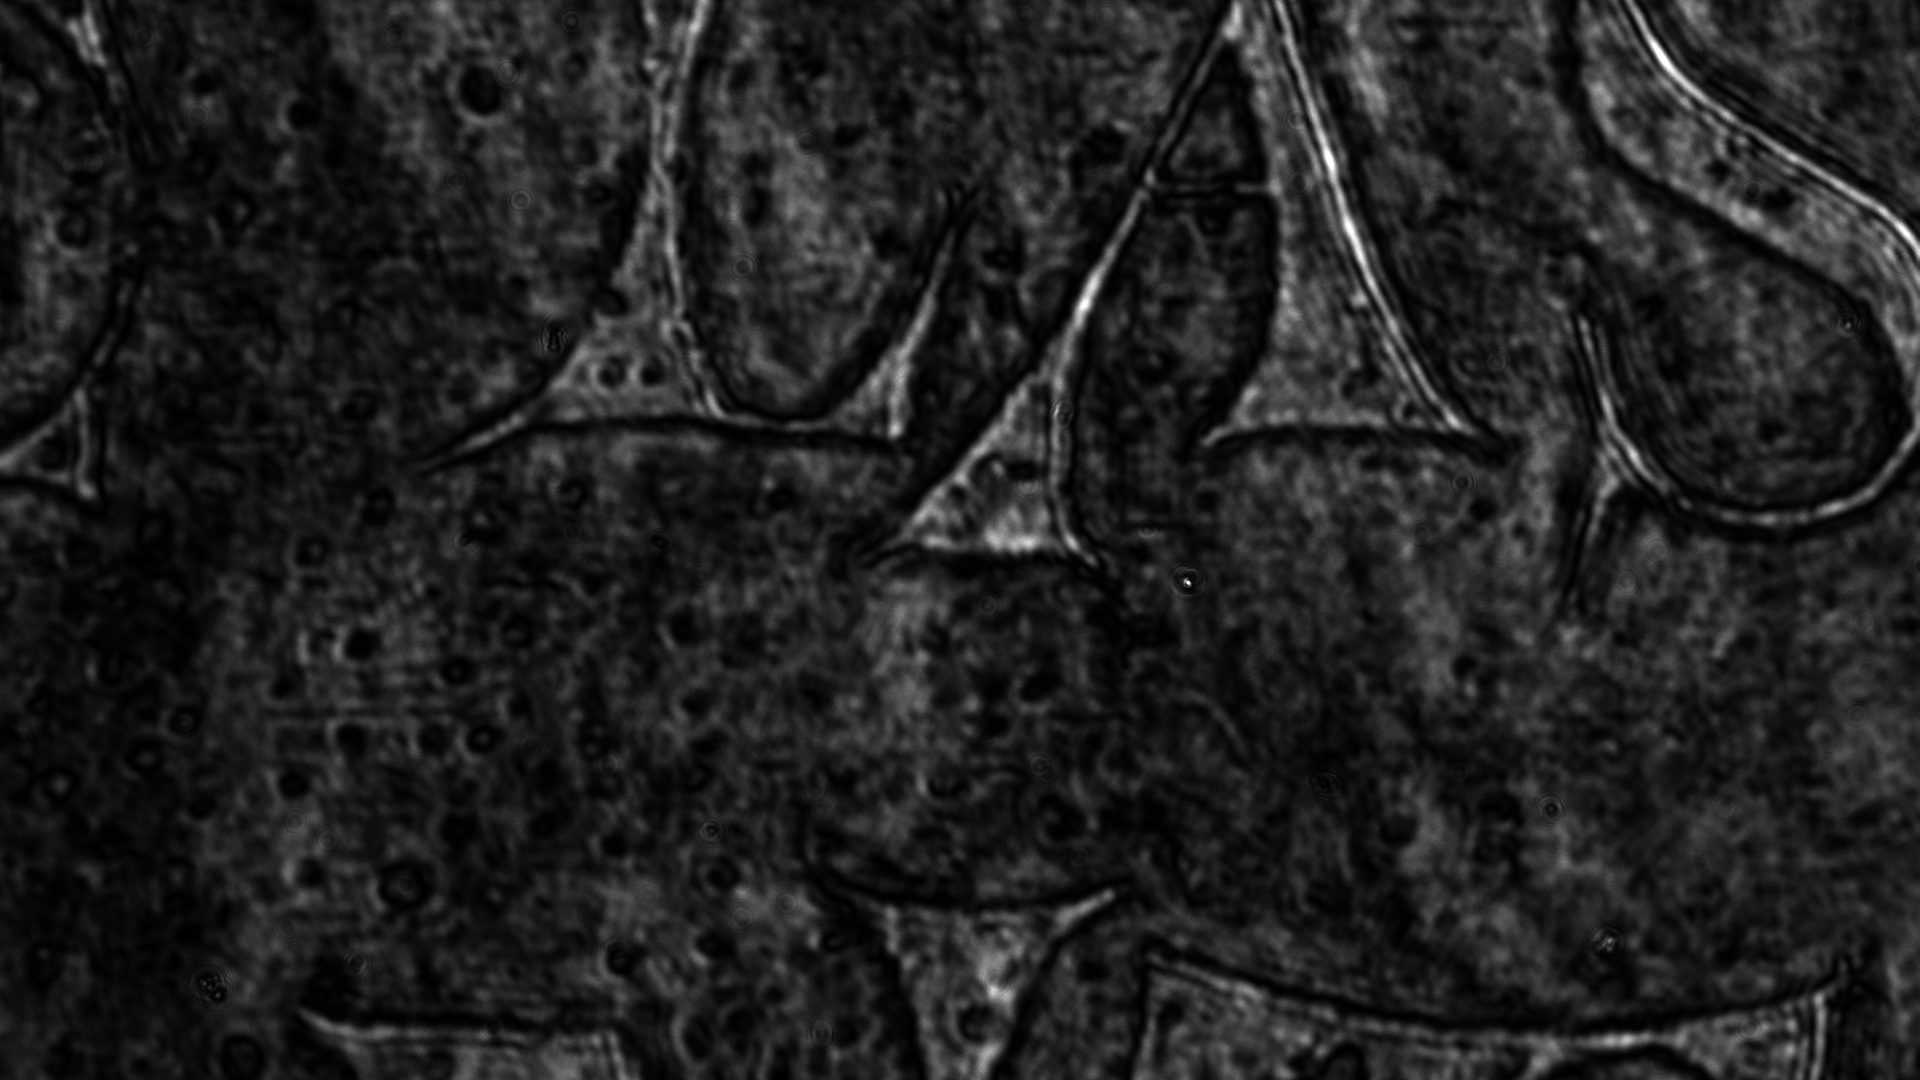
\includegraphics[width=\textwidth]{/parte4-filtrado/4f-pic-2ocm-diafragm-10cm-camera-letters-diafragma_y_punto-pasabanda.png}
%    \caption{que es }
%    \label{fig:filtrado1}
%   \end{subfigure}
%	\begin{subfigure}[t]{0.45\textwidth}\centering
%		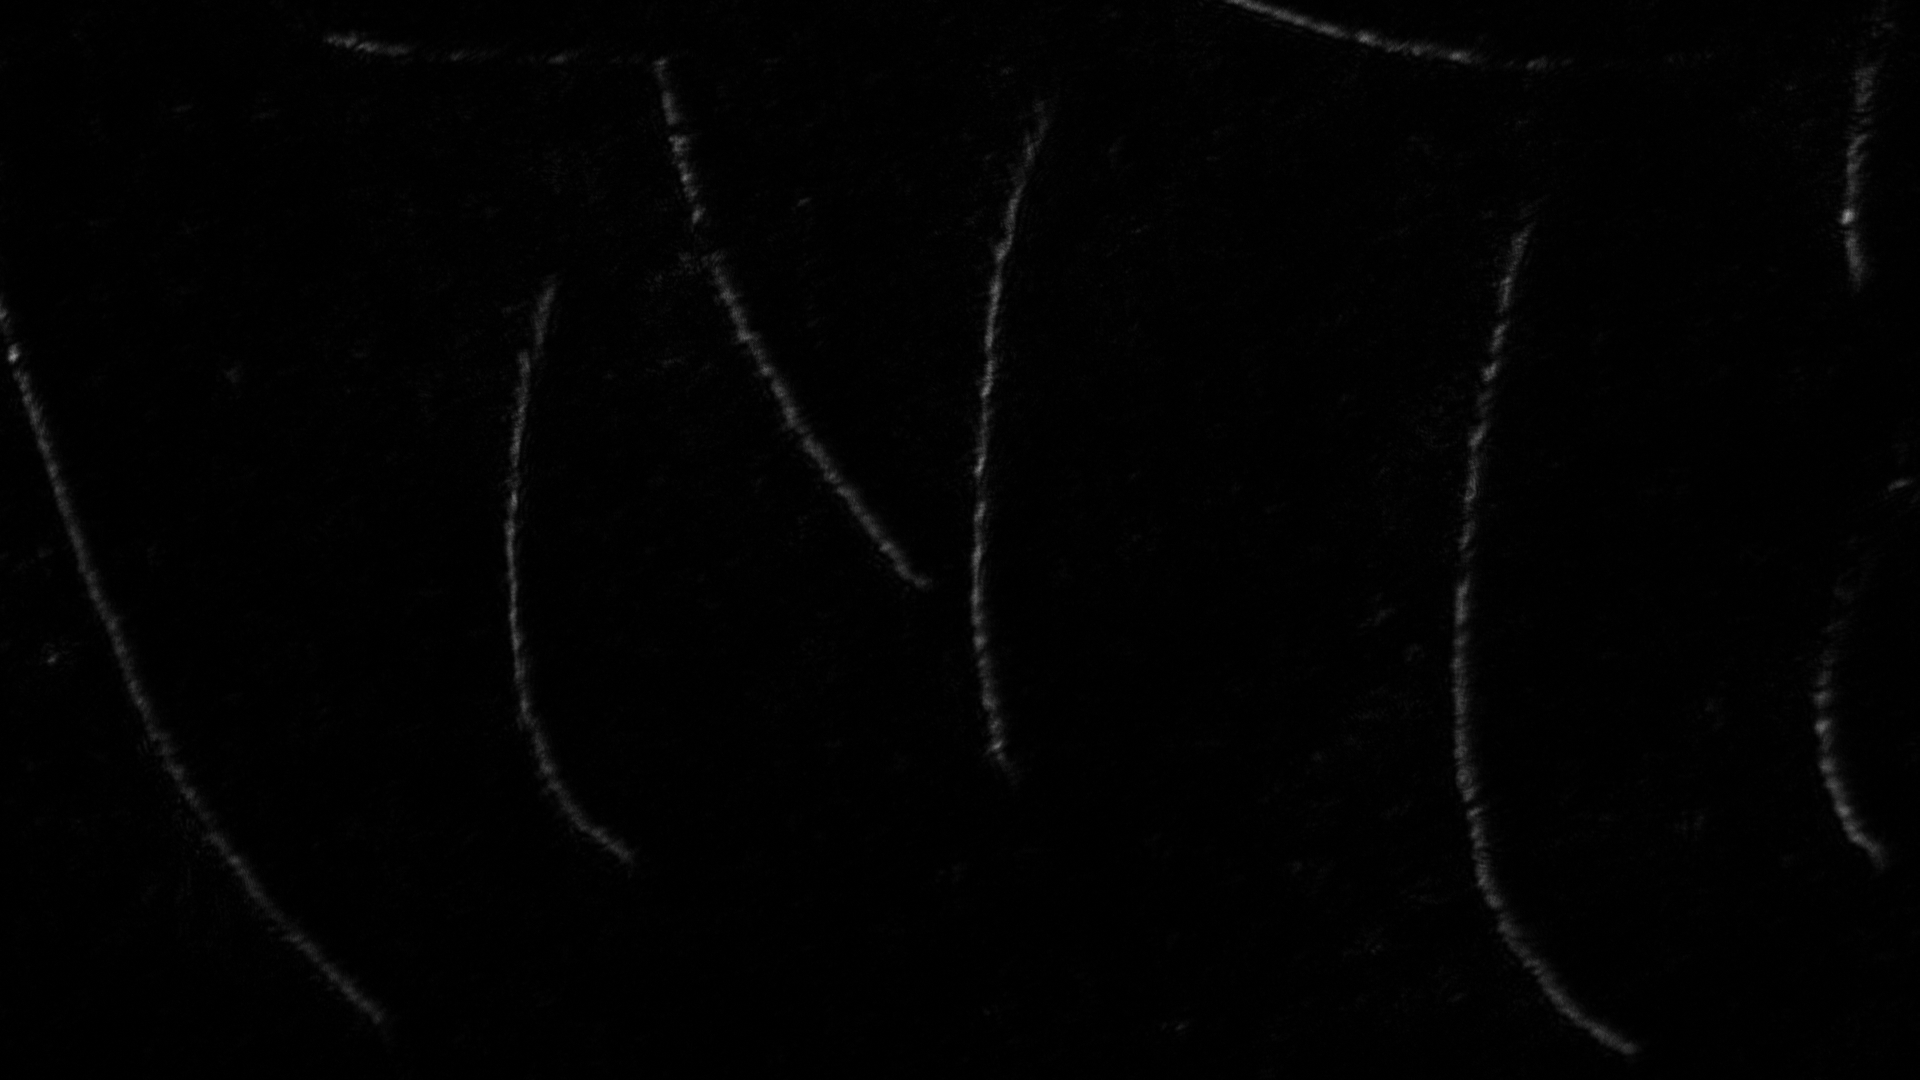
\includegraphics[width=\textwidth]{/parte4-filtrado/4f-pic-2ocm-diafragm-10cm-camera-letters-high-frequency-almost-x.png}
   % \caption{que es }
%    \label{fig:filtrado2}
%	\end{subfigure}
%	\begin{subfigure}[t]{0.45\textwidth}\centerng
%		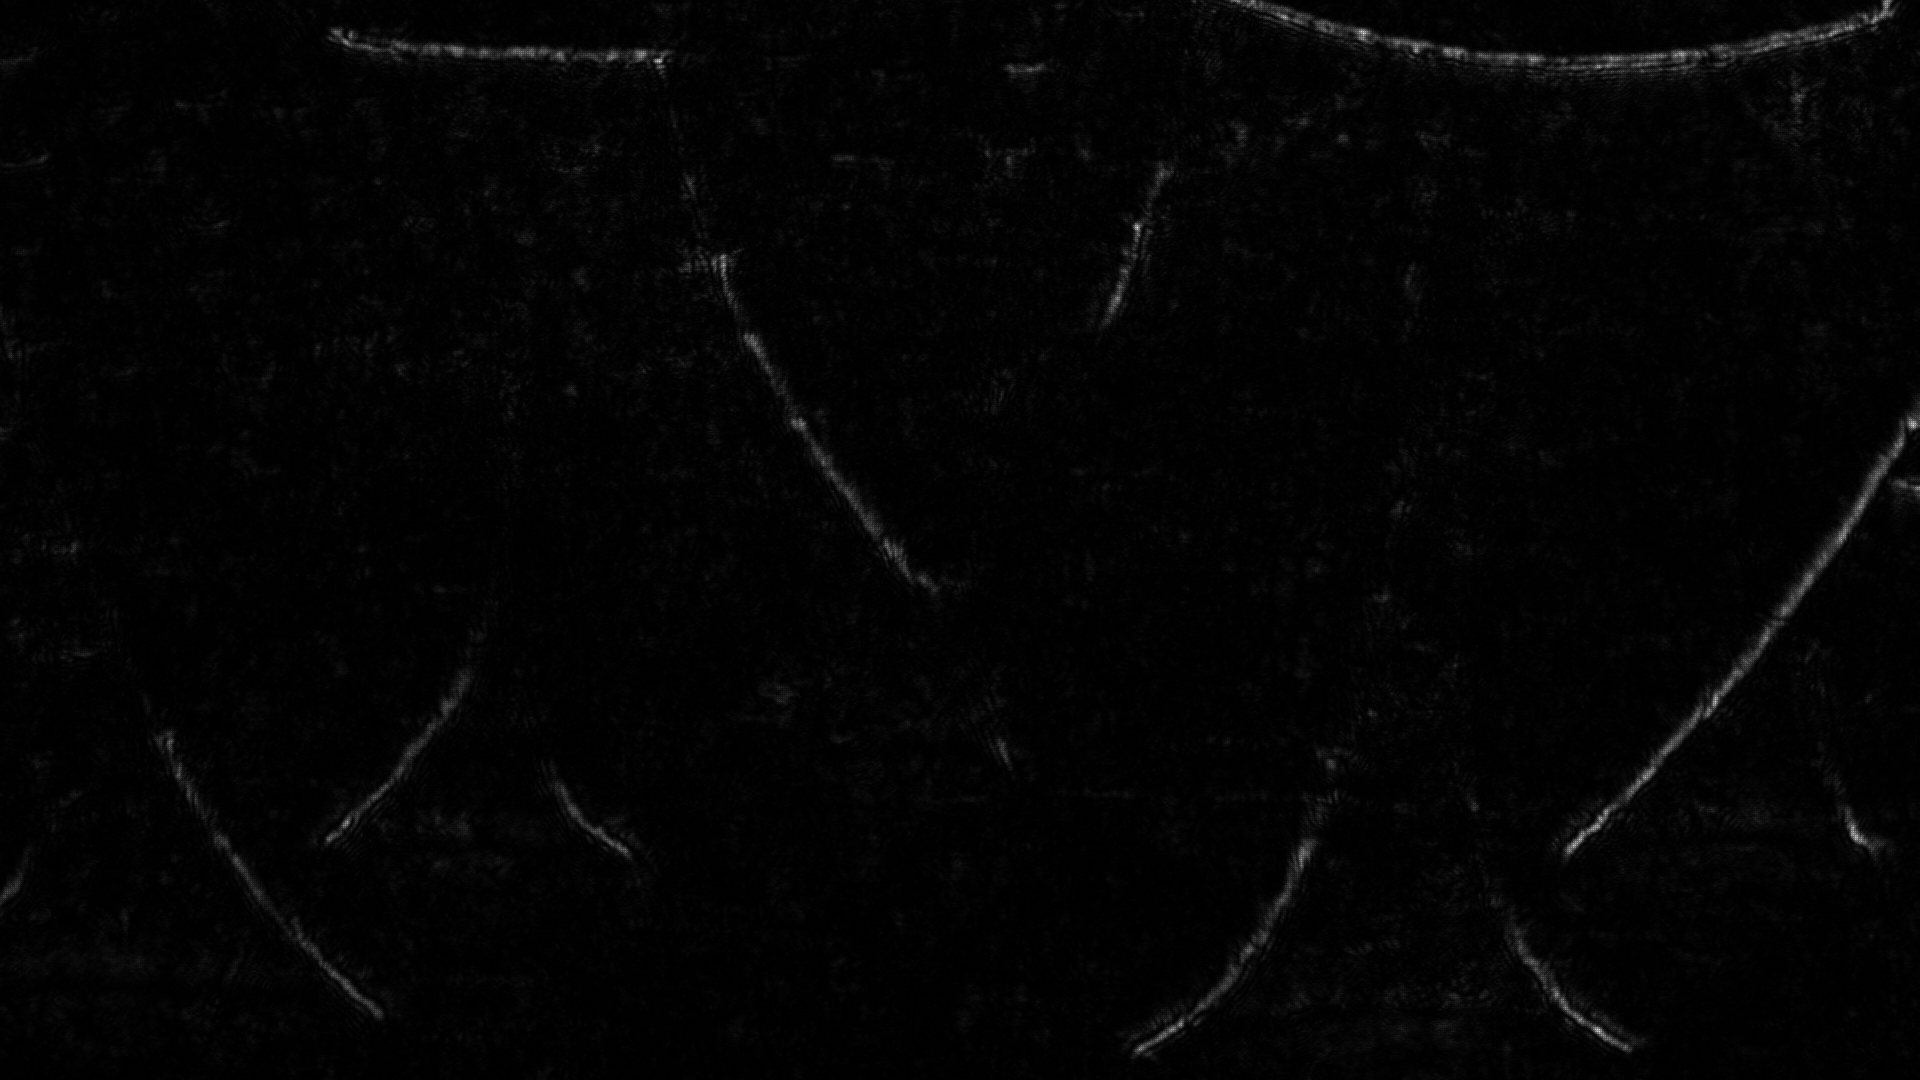
\includegraphics[width=\textwidth]{/parte4-filtrado/4f-pic-2ocm-diafragm-10cm-camera-letters-high-frequency-dot-down.png}
 %   \caption{que es}
 %  \label{filtrado3}
%	\end{subfigure}
%	\hfill
%	\begin{subfigure}[t]{0.45\textwidth}\centering
%		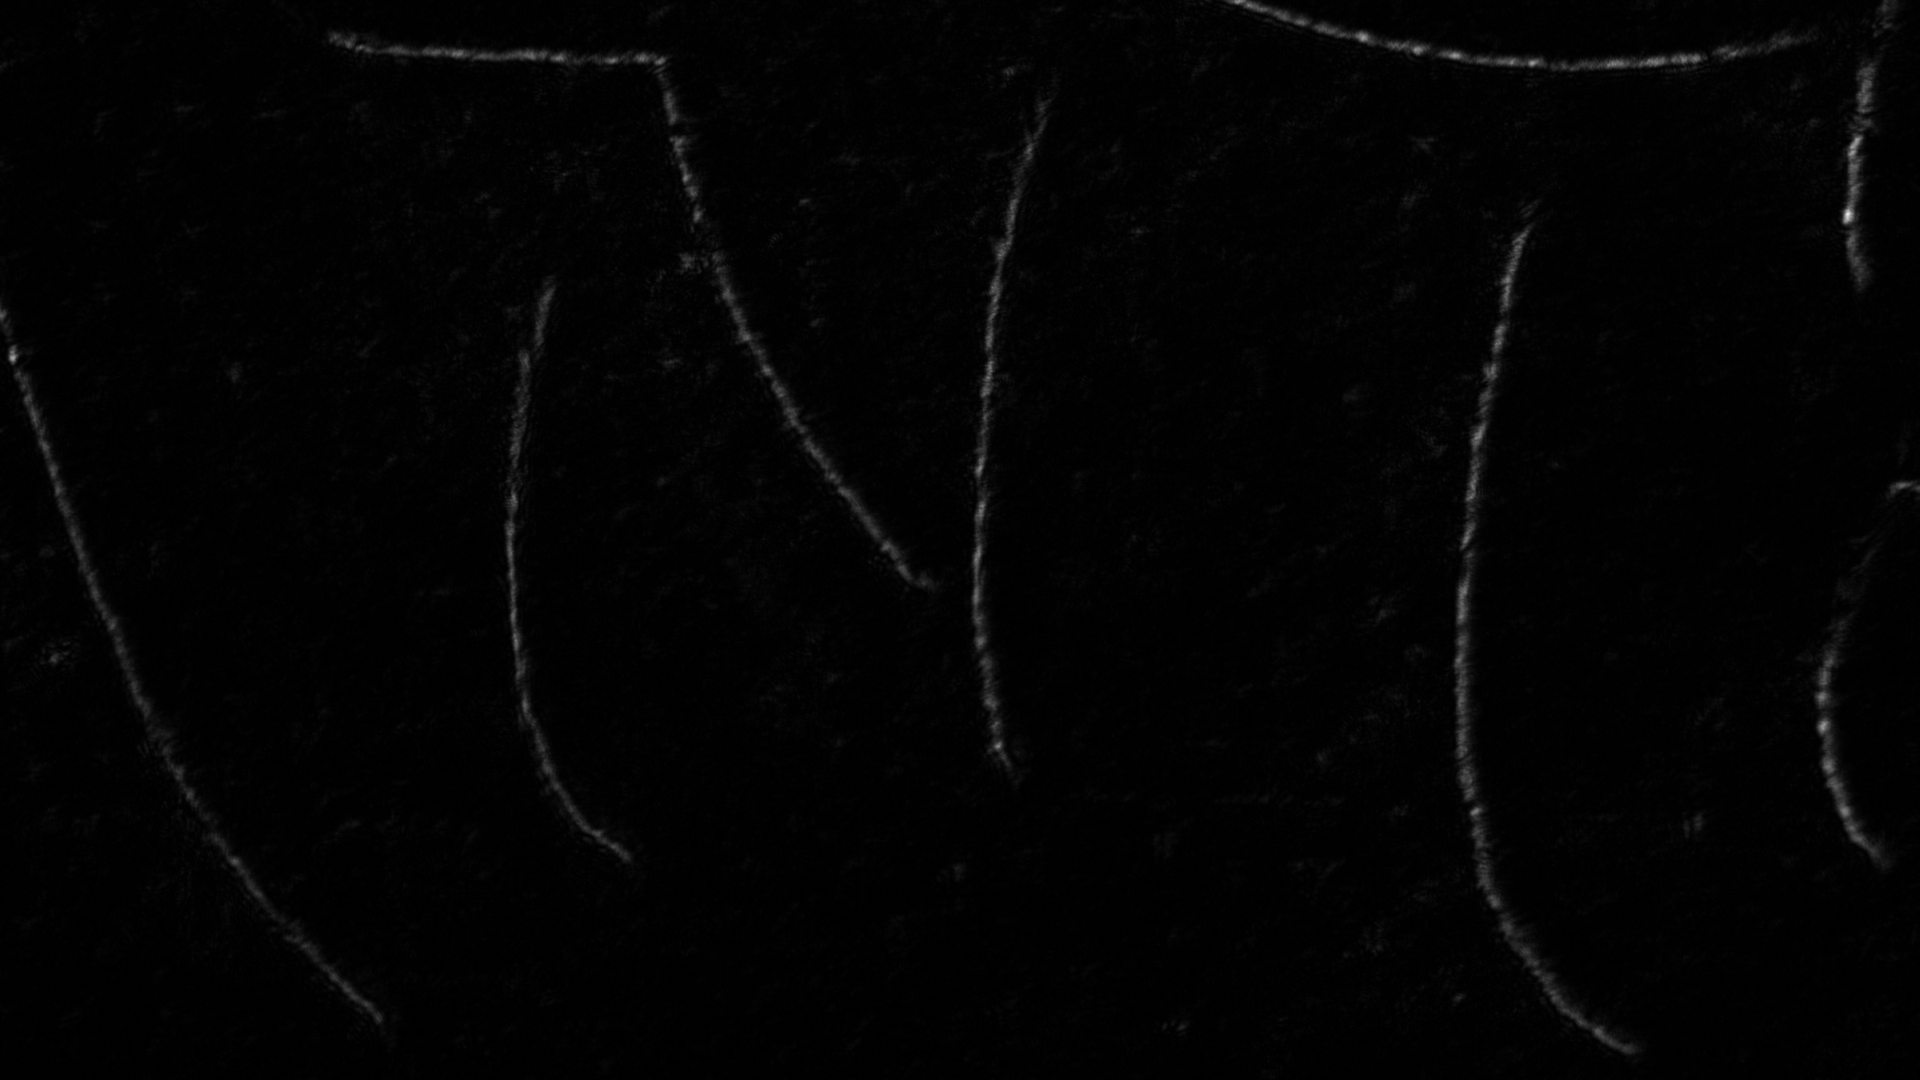
\includegraphics[width=\textwidth]{/parte4-filtrado/4f-pic-2ocm-diafragm-10cm-camera-letters-high-frequency-dot-right-a-bit-down.png}
 % \caption{que es }
 %	\end{subfigure}
%	\caption{que es}
%	\label{fig:filt}
%\end{center}
%\end{figure}

CUESTIONES:
\begin{enumerate}
\item ¿Qué distancia focal tiene la lente más próxima a la camera? Justifique el procedimiento seguido para determinar el orden de las lentes.
\item Elegir un filtro entre los estudiados en la práctica que podría ser adecuado para la observación de objetos semi-transparentes. Justifique la respuesta.
\item ¿Qué observamos en la salida del sistema si usamos como filtro una red periódica? Justifique la respuesta.
\end{enumerate}


\subsection{Formación de imágenes con luz parcialmente coherente}

CUESTIONES:
\begin{enumerate}
\item ¿El rango de distancias donde observamos la imagen del objeto 2D es mayor en el caso iluminación coherente o parcialmente coherente? ¿Qué iluminación es mejor para la observación de objetos 3D?
\item Para el sistema de filtrado usado en la práctica, la última lente es la pupila de salida del sistema. Determinar la respuesta impulsional y la función de transferencia del sistema en el caso de iluminación (a) coherente; (b) incoherente.

\end{enumerate}

\section{Conclusiones}

%%%%%%%%%% If using BibTeX:
\bibliography{bibliography}

\end{document}
